\documentclass{LSkill} 

\usepackage{hyperref} 
\usepackage{graphicx} 
\usepackage{amsmath}   
\usepackage{amssymb}   

% Title ,Subtitle, author and date
\title{Project 2-1 \\ \large{---}} 
\author{
    Cem Andrew Gültekin, Antonie Bostan, Vincent Helms, Mikle Kuzin, \\ 
    Kamil Lipiński, Calin Suconicov, Greg Vadász
}
\date{\today}

\begin{document}


\maketitle
\tableofcontents

% Abstract
\begin{abstract}
Multi agent training is a specific branch of reinforcement learning in which a group of agents are trained to achieve a task together. What this means, is that the performance of agents are measured by group, and not by personal performance. Their policies are also collective. This style of reinforcement learning allows researchers to implement studies on team-based games, such as football, which is what this study will be investigating. The study will look to optimize the learning of agents with realistic sensors to score goals in a 2 versus 2 format, based on the POCA algorithm. 
\end{abstract}

% Introduction
\section{Introduction}
The primary objective of this study is to identify the most optimal configuration for training a set of agents to play football using POCA using the unity platform. The POCA algorithm was chosen due to its capability to efficiently support multi-agent learning. Thus, the primary research question for this study is “How can the training of agent clusters using POCA be optimized in order to teach them to play football in unity?”.

However, this question is quite broad as there is a lot to cover under the umbrella of optimising a reinforcement learning algorithm for training agents for a specific task. Therefore, these researchers have decided to break down this broad primary research question into three sub-questions, each exploring a different aspect of this optimization. The three questions are; What is the most suitable set of values for the configuration file of a POCA training algorithm for this task? What is the optimal combination of realistic sensors for performance for this task? Does training in the unity editor alter the performance of the agents when compared to training in a pre-compiled file? 

When researching the topic of Multi Agent Reinforcement Learning (MARL), we found that the majority of studies were fairly broad, and few focused on optimising MARL for a very specific, niche task such as playing football. Studies such as  (L. Bus¸oniu et al., 2008)\cite{busoniu2008survey} and many more carry out much larger analyses on MARL as a whole, without diving into the specifics of POCA, especially not for a single task. In the field of MARL for football, we were able to find one single study which utilised PPO for a full 11 versus 11 football match simulation \cite{smit2023scaling_marl}. However, although PPO has been described as an effective MARL algorithm, it was not the algorithm’s original purpose \cite{yu2022ppo_cooperative}. Thus, we believe that by attempting to reconfigure the football game to be a 2 versus 2 scenario, as well as using the POCA algorithm instead of the PPO algorithm, we will be contributing something new to the MARL field of study.


In this study, we aim to discover if we can improve the football playing abilities of 4 agents in a 2v2 closed pitch scenario. We aim to do this using a POCA reinforcement learning algorithm, giving the agents both positive and negative rewards for certain actions. Ideally, as the agents experience playing they develop strategies to maximize the amount of positive rewards that they receive, using the POCA algorithm. We could not find any studies related to the specific task of training agents to play football using a POCA algorithm, thus we believe that our paper will be a novelty in this sense. As this study will be breaking down and exploring a very niche facet of multi-agent reinforcement learning, we believe that this study will be contributing to the current academic state of the art of reinforcement learning. 



In this study, we aim to discover if we can improve the football playing abilities of 4 agents in a 2v2 closed pitch scenario. We aim to do this using a POCA reinforcement learning algorithm, giving the agents both positive and negative rewards for certain actions. Ideally, as the agents experience playing they develop strategies to maximize the amount of positive rewards that they receive, using the POCA algorithm. We could not find any studies related to the specific task of training agents to play football using a POCA algorithm, thus we believe that our paper will be a novelty in this sense. As this study will be breaking down and exploring a very niche facet of multi-agent reinforcement learning, we believe that this study will be contributing to the current academic state of the art of reinforcement learning. 

\section{Methods}
In order to determine the most effective configuration of our training, we decided to use an Elo rating system. Out of all possible metrics we chose Elo rating as it is a very objective look at the performance of agents, which is the ultimate goal of this study. 
The reason why Elo rating is more compatible than some other measure such as cumulative reward is the fact that Elo shows the general progression of the agents’ policies as compared to previous policy versions. The logic behind this is explained in the Implementation section. 
	By comparing the teams over multiple iterations, we can see how the reinforcement learning policies develop, and whether they are improving when compared to previous versions. Thus, Elo rating is an effective and reliable way to measure the improvement of the reinforcement learning policies overtime that the training algorithm develops. 
	We used the Elo measurements provided by our POCA algorithm as a way of measuring the progress of the agent groups. More Elo progression meant better policy development, thus more optimal learning.

\begin{figure}[htbp]
    \centering
    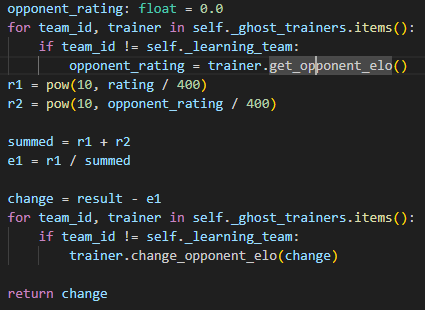
\includegraphics[width=0.5\textwidth]{figure 1.png} 
    \caption{Formula Of Elo Calculation}
    \label{fig:Formula Of Elo Calculation}
\end{figure}
By comparing the teams over multiple iterations, we can see how the reinforcement learning policies develop, and whether they are improving when compared to previous versions. Thus, Elo rating is an effective and reliable way to measure the improvement of the reinforcement learning policies overtime that the training algorithm develops. 
We used the Elo measurements provided by our POCA algorithm as a way of measuring the progress of the agent groups. More Elo progression meant better policy development, thus more optimal learning. 



\subsection{Method for Learning Algorithm Parameters Testing}
To find the optimal parameters of a learning algorithm like POCA we make runs with one parameter changed each time. Before the run we change the parameter we would like to make tests on from the configuration file (SoccerTwos.yaml in this case). For our tests we tested each parameter 3 times with the default value, a higher value and a lower value. For example hidden units:  256,  512,  1024. With 512 being the default. For each comparison the number of steps were kept the same.

\subsection{Methods for in-editor vs pre-compiled training comparison}
In this experiment, we use previously found optimal parameters.

In order to run the in-editor training, we have to run a command in the terminal: 
\texttt{mlagents-learn (path to)SoccerTwosBest.yaml --run-id=run\_1\_in\_editor}. We have to specify the path to the yaml file responsible for the training (\texttt{SoccerTwosBest.yaml} in this case). We also need to give a name to the run\_id. We call one training \texttt{run\_1\_in\_editor} and the second one \texttt{run\_2\_in\_editor}. When we enter the command, we run the scene in the Unity Editor.

In order to run the pre-compiled training, we first compile the Unity scene that we want to train the ML agents on into an executable file. To do this, we open the Unity Editor, go to \texttt{File -> Build Settings… -> Add open scenes}, and add the correct scene - \texttt{SoccerTwos} in this case. Then we click Build. We have to choose a folder in which the executable scene will be stored. 
We created a new folder called \texttt{Build} and chose this folder. 

Next, the scene is compiled. When it is ready, we have to run a command in the terminal: \texttt{mlagents-learn (path to) \textbackslash SoccerTwosBest.yaml --env (path to) \textbackslash UnityEnvironment.exe --run-id run\_1\_pre\_compiled --no-graphics}. We have to specify the path to the yaml file responsible for the training (\texttt{SoccerTwosBest.yaml} in this case) and the path to the executable environment (\texttt{UnityEnvironment.exe} in our case). We also need to give a name to the run\_id. We call one training \texttt{run\_1\_pre\_compiled} and the second one 
\texttt{run\_2\_pre\_compiled}. We also used \texttt{--no-graphics}, so the graphics 
of the scene are not generated, saving some computational power.

\subsection{Method for Sensor Testing:}
In order to compare the performances of different sensors, an in-editor training setup with the hyperparameters previously acquired were used. Three different sensor configurations were compared; Ray perception only, sound sensor only, ray perception and sound sensor combined. The ray perception sensor was a series of rays connected to the agent in a 120 FOV, in order to simulate realistic vision for the agent. The sound sensor was set up as an audio listener within the game with a set radius of 15 units. The ball was set to trigger a noise when it came into contact with an agent or a ball. The agents were then notified of this noise. Logically, when combined, the sensors would constitute the two most important senses of a football player. Hearing and sound. Thus this configuration would produce the best results. In order to compare how individual configurations of the sensors perform we ran a training set using the POCA training algorithm for 2 million steps for each algorithm. This way, all configurations could be compared in an objective manner side by side. 
	Elo rating is a viable way to compare how sensor types perform because certain sensor types should see faster progression in Elo rating than others. For example, we expected the sound sensors to have lower levels of Elo development, as it would take longer for agents to figure out what was happening in the beginning, thus leading to more ties. Ties should not influence Elo too much. 

\section{Implementation}
\subsection{POCA Function}
The MA-POCA(Multi Agent POsthumous Credit Assignment) algorithm was developed by unity’s ml agents team specifically for the purpose of training agents in a multi-agent setting. This algorithm is specially suited for MARL because of its centralized critic. What this means is that instead of each agent having their own individual policy creation, the centralized critic is able to evaluate the performance of the team as a whole, and create policies for each individual agent based on the performance of the team \cite{cohen2022absorbing_states}. The individual agents can still have their own unique rewards, although in our experiments this is not the case.

This central critic allows for interplay between agents seeking the same goal, such as football teammates, which makes POCA very suitable for teaching agents how to play team based sports. 
\subsection{Reward System}
We wanted to avoid overcomplicating our rewards system. We believe that if we rewarded too many behaviors among our agents, we would risk the policies overfitting on a certain action that is not conducive to the ultimate goal of the agents, which is to score goals.
This meant that we chose to only reward agents for their goal scoring, as well as give them a negative reward for conceding a goal, thereby making the ultimate focus on the game objective. Additionally, there was a small constant negative reward for agents as long as no goal was scored, to ensure that the game did not become stagnant, as well as to ideally increase the rate at which goals were scored. This does mean since there was no specific guidance for the agents as they developed their initial policies, because the idea of scoring on the goal object is very vague, and not something that is easily determinable. Thus, we expected initial progress to be slower. 

What helped in this scenario is that the field was of a relatively small size when compared to our agents, ball and goal post which meant that the likelihood of scoring early on by accident was high. This would allow the agents to start developing their policies in the right direction. 
\subsection{Elo System}
The Elo system in this training setup was based around the fact that football is a zero sum game. Thus, one team always has to win and one team has to lose, or they can draw. This means that both teams have their own respective Elo which gets changed after every round, determined by either a goal or time running out. The Elo is adjusted relative to the Elo of the other team. If the Elos are similar in value, the win is considered more valuable than if the opposing team’s Elo is much lower than the winning team’s. The reverse goes for a loss. 

This system is incorporated into the training system in order to track policy progression. The team being trained gets their policy updated every round, whereas the opposing team (ghost team) has a policy which gets changed less frequently. Specifically, the policies of the ghost team are derived from a previous policy of the training team. The ghost team has a bank of old policies which it can rotate through, so that the training team doesn’t overfit to only beat one old policy. 

The idea behind using old policies to compare new policies, is that as the agents are developing their policies, they should be better than their previous versions. Thus, decreasing Elo indicates that policy development is making the agents worse overtime, whereas increasing Elo suggests that the policies are developing well, and beating their previous versions. 

The logic of the Elo calculation is the following:

\[
E_A = \frac{1}{1 + 10^{(R_B - R_A)/400}}
\]

\par % Adds a paragraph break
Where \(E_A\) is the expected score of team \(A\) and \(R_X\) is the Elo score of team \(X\).

\[
R_A' = R_A + K(S_A - E_A)
\]

\par % Adds space between the equations
Where \(R_A'\) is the new score of team \(A\), \(K\) is the K-factor, and \(S_A\) is the performance of team \(A\), which is either 1 for a win or 0 for a loss. Draws are not considered in Elo rating.

    

%EXPERIMTENS    
\section{Experiments}

We have employed Bayesian optimization, facilitated by the Optuna framework, to automatically tune the hyperparameters of the PPO algorithm. The core objective was to maximize the Elo rating achieved by trained agents, serving as a proxy for overall performance within the game. The implementation leveraged a modular design, comprising several key stages:

\subsection{Configuration Generation and Dynamic Parameterization}

A base configuration file, specified in YAML format, defined the core structure and parameters of the PPO agent. A \texttt{create\_temp\_trainer\_config} function dynamically modified this configuration based on hyperparameters proposed by Optuna. Specifically, the following hyperparameters were included in the search space:

\begin{itemize}
    \item \textbf{learning\_rate}: A continuous parameter controlling the step size of the optimizer, sampled logarithmically between \texttt{1e-5} and \texttt{1e-3}.
    \item \textbf{batch\_size}: A categorical parameter defining the size of mini-batches used in the optimization process, selected from options \{\texttt{512}, \texttt{1024}, \texttt{2048}\}.
    \item \textbf{buffer\_size}: A categorical parameter that governs the size of the experience replay buffer, with options \{\texttt{2048}, \texttt{4096}, \texttt{8192}\}.
    \item \textbf{beta}: A continuous parameter defining the strength of the entropy bonus, sampled between \texttt{0.0001} and \texttt{0.01}.
    \item \textbf{num\_layers}: An integer parameter specifying the number of layers in the neural network, with options \{\texttt{1}, \texttt{2}, \texttt{3}\}.
    \item \textbf{hidden\_units}: A categorical parameter defining the number of hidden units in each layer, with options \{\texttt{128}, \texttt{256}, \texttt{512}\}.
\end{itemize}

These hyperparameter suggestions were integrated into a modified configuration file, which was stored temporarily for use in each trial. This approach allowed for iterative exploration of the hyperparameter space, with each trial using unique settings.
\subsection{Training and Performance Evaluation}

The \texttt{run\_training\_and\_get\_score} function executed the training process using the \texttt{mlagents-learn} command-line tool. The generated temporary configuration was provided as an argument, along with the path to the simulation environment. To manage resources and monitor the training, the following steps were taken.

The training progress was logged to a console output file, enabling retrospective analysis of the training process as well as providing key performance metrics, as the version of the ML-Agents we were using didn’t have proper support to parse the TensorBoard files in runtime.

The training procedure was set for a predefined duration of 500,000 steps in each trial. The \texttt{parse\_from\_console} function then analyzed the console output log, extracting the final Elo rating achieved by the trained agents. This metric served as the objective function to be maximized by the Bayesian optimization process.
\subsection{ Bayesian Optimization and Iterative Search:}
The Optuna framework's Bayesian optimization algorithm, which uses a Gaussian process as a surrogate model of the objective function, was applied to iteratively explore the hyperparameter search space.

A study was established using the SQLite storage backend to store the history of trials, allowing for continuation of optimization if necessary. The direction of optimization was set to "maximize", in order to achieve the highest ELO value as the desired outcome.

The objective function consolidated the configuration generation, training execution, and performance evaluation phases. After each trial was finished, the temporary configuration file was deleted to maintain a clean working directory.

The best result was saved and outputted to the console including the ELO and the hyperparameters that produced that result.

The script was run until for 10 consecutive runs no improvement could be noted and resulted in the following hyperparameters:


\begin{verbatim}
    batch_size: 512
    buffer_size: 4096
    beta: 0.0020460882794934116
    hidden_units: 512
    num_layers: 1
\end{verbatim}

\subsection{Finding The Optimal Learning Rate}
Our second experiment is making 3 runs with different learning rates in the SoccerTwos environment. The goal is to find the optimal learning rate by examining the models performance, convergence speed, CPU/GPU usage and framerate of the simulations. The 3 learning rates are 0.0001, 0.0003 and 0.0009. The runs will be examined until 3.5 million steps.

\subsection{Finding The Optimal Hidden Unit Number}
Our third experiment is making 3 runs with different hidden unit numbers in the SoccerTwos environment. The goal is to find the optimal hidden unit number by examining the models performance, convergence speed, CPU/GPU usage and framerate of the simulations. The 3 hidden unit numbers are 256, 512 and 1024.
 
\section{Results}
\subsection{Finding The Optimal Learning Rate}
As shown in Figure~\ref{fig:Cumulative Reward For Learning Rates}, the learning rates from grey to orange are 0.0009, 0.0003 and 0.0001. It takes 320 thousand steps for 0.0009 to get to max cumulative reward. 510 thousand steps for 0.0003 and 640 thousand for 0.0001.

So the learning rate of 0.0009 was able to reach the maximum cumulative reward significantly faster than the rest. The 0.0001 learning rate took the longest and 0.003 was somewhere between. And all of the learning rates converged before 650 thousand steps.


\begin{figure}[htbp]
    \centering
    \includegraphics[width=0.5\textwidth]{figure 2.png} 
    \caption{Cumulative Reward For Learning Rates}
    \label{fig:Cumulative Reward For Learning Rates}
\end{figure}

If we look at Figure~\ref{fig:ELO For Learning Rates} which shows us how the ELO changes throughout the run we can see 0.0009 starts well compared to the others. After 500 thousand steps each of the learning rates increase their elo steadily almost at the same rate. So at the end at 3.5 million steps the results are the same as the beginning.

\begin{figure}[htbp]
    \centering
    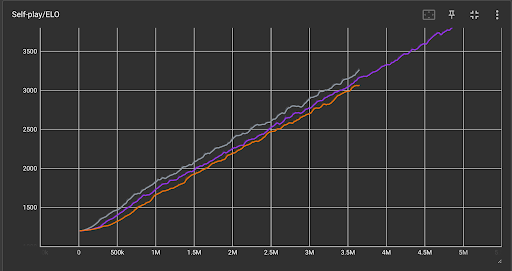
\includegraphics[width=0.5\textwidth]{figure 3.png} 
    \caption{ELO For Learning Rates}
    \label{fig:ELO For Learning Rates}
\end{figure}

Now if we look at Figure~\ref{fig:Baseline Loss For Learning Rates} for the baseline loss we can see 0.0009 is the first to converge to the final range. After that 0.0003 is the second and 0.0001 is the last.

\begin{figure}[htbp]
    \centering
    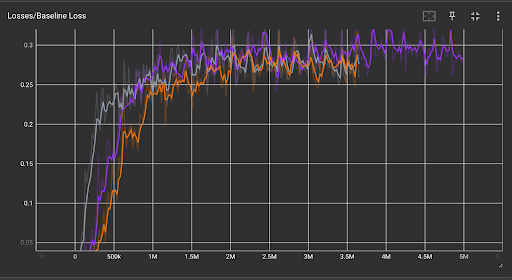
\includegraphics[width=0.5\textwidth]{figure 4.png} 
    \caption{Baseline Loss For Learning Rates}
    \label{fig:Baseline Loss For Learning Rates}
\end{figure}
\vspace{1cm}

There wasn’t much of a difference in the time it took for 3.65 million steps. 

\begin{verbatim}
	0.0009 learning rate took 6.872 hr
	0.0003 learning rate took 6.203 hr
	0.0001 learning rate took 6.999 hr
\end{verbatim}

	Frame Count in 3.65 million steps:

\begin{verbatim}
	0.0001 learning rate 548862 frames
	0.0003 learning rate 547517 frames
	0.0009 learning rate 547493 frames
\end{verbatim}

If we look at the CPU Usage on scripts and rendering both 0.0001 and 0.0009 learning rates have a lot of spikes in ms throughout the run. They jump to 66ms(15FPS) from 33ms(30FPS). While the run with 0.0003 mostly stays around 33ms(30FPS).
(APPENDIX A)
\vspace{0.5cm}

At Figure~\ref{fig:CPU Performance For Learning Rates} we have the CPU processing times from the main thread at the last frame of each run. The total CPU frame time is lowest at 0.0003 learning rate with 627.10ms making it the most efficient. The longest total CPU Frame time is at 0.0001 learning rate with 935.45ms. But it has the lowest number in the other 3 categories with most of its time on Render Loop.

\begin{figure}[htbp]
    \centering
    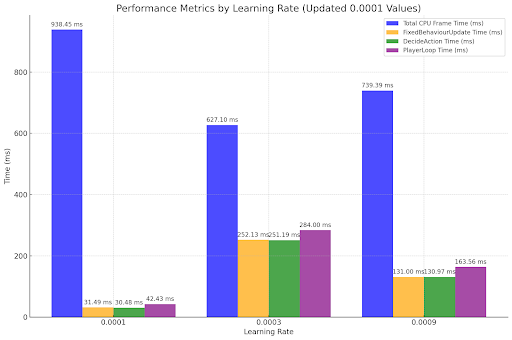
\includegraphics[width=0.5\textwidth]{figure 5.png} 
    \caption{CPU Performance For Learning Rates}
    \label{fig:CPU Performance For Learning Rates}
\end{figure}
\vspace{0.5cm}
Finally if we look at the memory usage of all at Figure~\ref{fig:Total Commited Memory By Learning Rates}. We can see that there is no significant relation between the learning rate and total committed memory.

\begin{figure}[htbp]
    \centering
    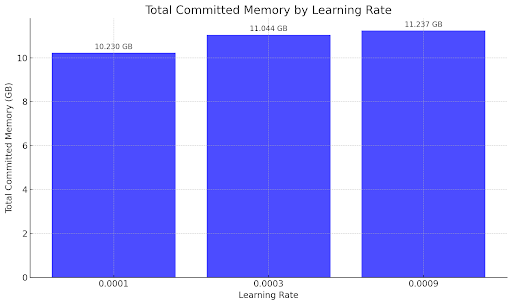
\includegraphics[width=0.5\textwidth]{figure 6.png} 
    \caption{Total Commited Memory By Learning Rates}
    \label{fig:Total Commited Memory By Learning Rates}
\end{figure}

\subsection{Finding The Optimal Hidden Unit Number}
To start with the cumulative reward if we look at Figure~\ref{fig:Cumulative Reward For Hidden Units} from orange to purple the hidden unit numbers go as 1024, 256 and 512. The run with 1024 hidden units is the first to converge at 320 thousand steps. After that the run with 256 hidden units converges at 510 thousand steps and the run with 512 units converges last at 520 thousand steps.

As we can see the run with 1024 units converges first but it suffers a big drop around 500 thousand steps. After that others converge before it can get back to maximum reward. But at the end all of them manage to converge around 500 thousand steps.

\begin{figure}[htbp]
    \centering
    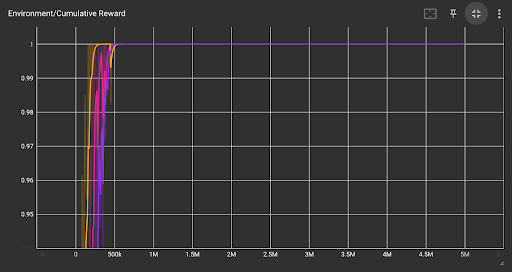
\includegraphics[width=0.5\textwidth]{figure 7.png} 
    \caption{Cumulative Reward For Hidden Units}
    \label{fig:Cumulative Reward For Hidden Units}
\end{figure}

Now if we have a look at ELO of the runs at Figure~\ref{fig:ELO For Hidden Units} the run with 1024 units starts off faster than the others and leads towards the end. After the start all of them continue to rise steadily at the same pace. So at the end they have very similar ELO’s. At 3.65 the highest elo is at 1024 units and the lowest is 512.

\begin{figure}[htbp]
    \centering
    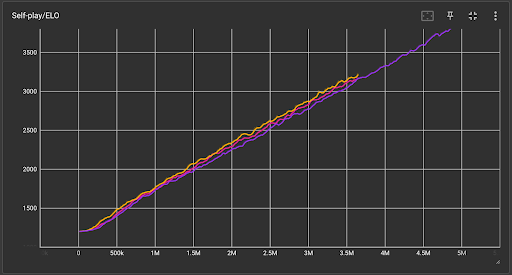
\includegraphics[width=0.5\textwidth]{figure 8.png} 
    \caption{ELO For Hidden Units}
    \label{fig:ELO For Hidden Units}
\end{figure}

When we look at Figure~\ref{fig:Baseline Loss For Hidden Units} for Baseline Loss the first to converge to the final range is 1024 units and the last is 256 units.

\vspace{0.5cm}
\begin{figure}[htbp]
    \centering
    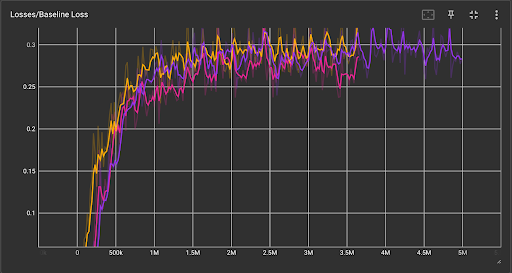
\includegraphics[width=0.5\textwidth]{figure 9.png} 
    \caption{Baseline Loss For Hidden Units}
    \label{fig:Baseline Loss For Hidden Units}
\end{figure}

Time difference for 3.65 million steps

\begin{verbatim}
    256 Hidden Units took 5.544 hr		
    512 Hidden Units took 6.169 hr
    1024 Hidden Units took  7.5 hr
\end{verbatim}

The time for the run increases significantly as the hidden units count increase.

Frame count for 3.65 million steps
\begin{verbatim}
    256 Hidden Units: 547497		
    512 Hidden Units: 547517
    1024 Hidden Units:547518
\end{verbatim}

If we look at the CPU usage on scripts and rendering, all of the hidden unit counts averages 33ms(30fps). But the number spikes to 66ms(15fps)  as the hidden unit counts go up. 
(Appendix A)

\vspace{0.5cm}

At Figure~\ref{fig:CPU Performance For Hidden Units} we have the CPU processing times from the main thread at the last frame of each run. The total CPU frame time increases significantly as the number of units increases. 256 units has the lowest frame time in all categories which means it is the most computationally efficient. While 1024 with all of the highest frame times is the least computationally efficient.


\begin{figure}[htbp]
    \centering
    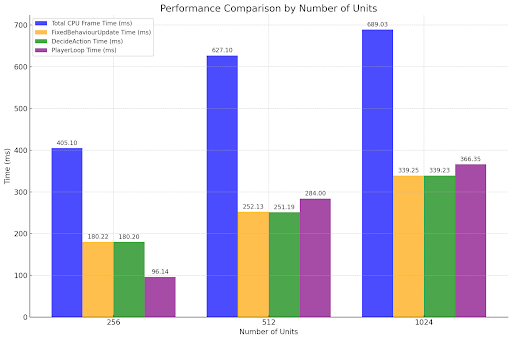
\includegraphics[width=0.5\textwidth]{figure 10.png} 
    \caption{CPU Performance For Hidden Units}
    \label{fig:CPU Performance For Hidden Units}
\end{figure}

Finally if we look at the memory usage of all at Figure~\ref{fig:Total Commited Memory By Hidden Units}. We can see that there is no significant relation between the number of hidden units and total committed memory.

\begin{figure}[htbp]
    \centering
    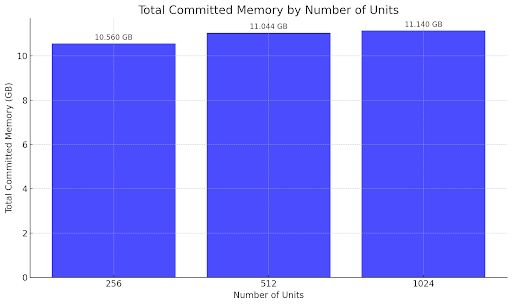
\includegraphics[width=0.5\textwidth]{figure 11.png} 
    \caption{Total Commited Memory By Hidden Units}
    \label{fig:Total Commited Memory By Hidden Units}
\end{figure}

\subsection{In-editor vs pre-compiled}
We run the pre-compiled training twice since it is very fast and the in-editor training once.
The results for pre-compiled training in the table below are the average from two runs. The measured values are:


\subsection{Sensor Results}

%Discussion
\section{Discussion}


\subsection{In-editor vs pre-compiled}
Training in a pre-compiled environment is significantly faster compared to in-editor training. Our experiment showed that it is almost 8 times faster. The ELO rating turned out to be a bit higher for in-editor training,however if we take into account the  performance/time metrics, then pre-compiled training is over 7 times more effective, achieving 70,6 ELO/minute average growth compared to 9,62 ELO/minute. The episode lengths of agents trained in-editor were shorter (29.5 s) compared to those in the pre-compiled environment (43.9 s). This difference may result from variations in environment dynamics, synchronization, or computation handling, suggesting that the pre-compiled setup may provide a more precise simulation of the agent's interactions. Both setups achieve the same cumulative reward (1), indicating that both methods are capable of achieving the desired reward, though other metrics differ. The pre-compiled setup shows slightly lower baseline loss (0.22) compared to the in-editor setup (0.26). Lower baseline loss may suggest better generalization or stability. Policy loss is very similar for both setups, with the in-editor setup having a slightly lower policy loss (0.031 vs. 0.033). This metric doesn't show significant differences. The pre-compiled setup has a lower value loss (0.20) compared to the in-editor setup (0.25), indicating better value function approximation. Resource usage analysis revealed significant differences in CPU and RAM consumption. The pre-compiled environment consumed more than twice the CPU power on average (21.80% vs. 8.28% in-editor), likely due to more intensive real-time computations. RAM usage differences were less pronounced, with the pre-compiled environment using 13.15% compared to 12.9% in-editor. The higher CPU usage in the pre-compiled environment likely contributed to its greater efficiency, making it a better option for fast agent training.
\subsection{Learning rate}
For our experiment in learning rate the cumulative reward results shows us that the run with 0.0009 learning rate converged to the maximum faster than the rest without showing many fluctuations meaning 0.0009 would be the optimal learning rate in this category. Same goes for the ELO as the run with the 0.0009 learning rate is slightly higher throughout the run from the others. Furthermore, the time it took for the runs until the same step didn’t change with the learning rate. And if we look at CPU frame time 0.0009 learning rate is in the middle indicating there isn’t a performance issue with it. But most importantly these results matched with our  Bayesian optimization we did earlier. With the optimization we got a learning rate of  0.0007968671455358874. Which is closest to our pick out of the 3 learning rates. This confirms our results are valid.
\subsection{Hidden units}
In our experiment with hidden units it follows a similar performance metric with the learning rate. The highest hidden units count(1024) is the fastest to converge to maximum cumulative reward. And it is the one with the highest ELO throughout the run. But in this case there were drawbacks in CPU usage and time efficiency. The run with 1024 hidden units had the most spikes in scripts and rendering. And had the worst CPU performance, with slower processing leading to longer run times. So in this case it is an argument of Performance/Efficiency, if we go in the middle with 512 hidden units we will get the same results as in our Bayesian optimization run. So in the end of our research we would go with 512 hidden units.
\subsection{Sensor Discussion}
What we can derive from the data of our experiments with sensors is that each individual configuration affects training and policy generation in a similar way. We found that the combined sensor configuration was the most balanced of the three configurations, and thus seems to be the most stable sensor configuration for long term training. We believe this because although the combined sensor had the lowest Elo rating, meaning it progressed more slowly compared to previous versions of itself, it had the lowest policy loss, and was the middle of the pack in cumulative reward generation. This makes sense, since this configuration provides the most data for the critic to determine optimal policy. 

When we compare this performance to our ray perception only configuration, we can see that although the Elo was the highest out of the three, the cumulative reward was actually negative, meaning that the agents presumably took very long to make goals, and most likely did not score goals in quite a few runs. The reasoning behind that assumption is that the agents could not have been conceding goals, since they were increasing in Elo, however the only way to lose reward without losing Elo is scoring few goals with long time differences between scores. The policy loss of the ray perception sensor was not significantly higher, indicating that the training policy may take longer to develop and have spikes of poor performance due to unreliability. 

Finally, when looking at the sound sensor only, we see that it had the highest cumulative reward, and the highest policy loss, with the second highest Elo rating. This indicates that this system may perform the best at scoring goals, however its training is the most unpredictable. This makes sense since it would be difficult to develop a reliable policy on aiming a ball into a goal, without knowing where the goal is. This means that the policy changes may have been more erratic in this configuration, leading to less predictable rounds. 
% Conclusion
\section{Conclusion}
\subsection{In-editor vs pre-compiled}
The results  show that the pre-compiled environment offers significantly higher training efficiency in terms of speed. It is much faster than the in-editor environment, achieving better efficiency metrics (ELO/min). With lower baseline loss and value loss, the pre-compiled environment may be more stable and provide better value function approximation, which makes it an ideal choice for creating a good model in a reasonable amount of time.
\subsection{Sensor}
Overall, the combined sensor configuration seemed to be the best for long-term training due to its low policy loss, and acceptable performance in self-play. 
% Bibliography

\bibliographystyle{unsrt}
\bibliography{selectionsortBib}
\section{Appendix}

\end{document}
